The goal of this section was to recover estimated costs for each bidder.

To simplify the conditional statements that we will have to make, we will only
focus on the most common auctions that have a particular pair of number of small
and large businesses. The largest sample in the Cal Trans data set is one small business
and three large businesses. % FIXME: elaborate on why we are doing this
Focusing on only one pair of \(n_S\) and \(n_L\) simplifies the calculation
of density functions.

As we found in the previous section, for small businesses:
\[
  c_i(b_i; E, n_S, n_L) = b_i - \left(\frac{(n_S - 1) \cdot g_S(\beta_S(c_i \mid E) \mid n_S, n_L)}{1 - G_S(b_i \mid n_1, n_2) \cdot} +
    \frac{(n_L) \cdot g_L(1.05 b_i \mid n_L, n_S)}{1 - G_L(1.05 b_i \mid n_L, n_S)} \right)^{-1}
\]
and for large businesses:
\[ 
  c_i(b_i; E, n_S, n_L) = b_i - \left(\frac{(n_S) \cdot g_S(\frac{1}{1.05} b_i \mid n_S, n_L)}{1 - G_S(\frac{1}{1.05} b_i \mid n_1, n_2) \cdot} +
    \frac{(n_L - 1) \cdot g_L(b_i \mid n_L, n_S)}{1 - G_L(b_i \mid n_L, n_S)} \right)^{-1}
\]
In these equations, \(g_s, G_s\), etc., represent the pdf and cdf of the bids.
To find them, we use the definition of conditional probability:
\[
P(A \mid B) = \frac{P(A \land B)}{P(B)}
\]
Therefore, we need to estimate densities for the joint probability of bids and
estimates and the marginal probability of estimates.

We will first estimate functions for the bids (i.e., \(g_s\) and \(g_l\)
in the above equation). They will be conditional on the engineers estimate.
To simplify this, we will condition on the median of the engineers estimate.
For our subset of the auctions with the most common combination of large/small bidders,
this was \$526000.

We will now estimate the PDF of small business bids which is conditional on the
median of the engineers estimate.
It will not be conditional on the number of small and large businesses because
we are fixing it to our chosen subset of auctions.

First, here are 3D plots of the conditional PDFs of bids on estimates, for
small and large businesses.
\begin{figure}[ht!]
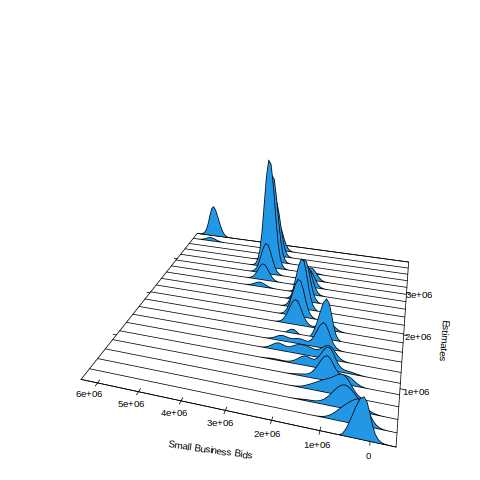
\includegraphics[scale=0.5]{imgs/g_s_cond.png}
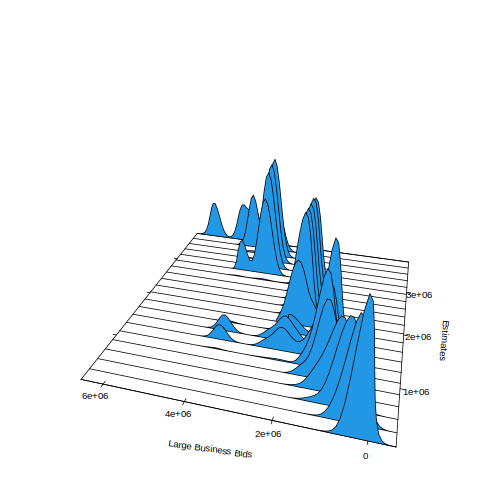
\includegraphics[scale=0.5]{imgs/g_l_cond.png}
\end{figure}

\newpage
Then, here are the graphs of the PDF for small/large businesses evaluated on their
bids, conditional on the median estimate from our subset (which is the same
for both large and small businesses, given they compete in the same auctions).
\begin{figure}[ht!]
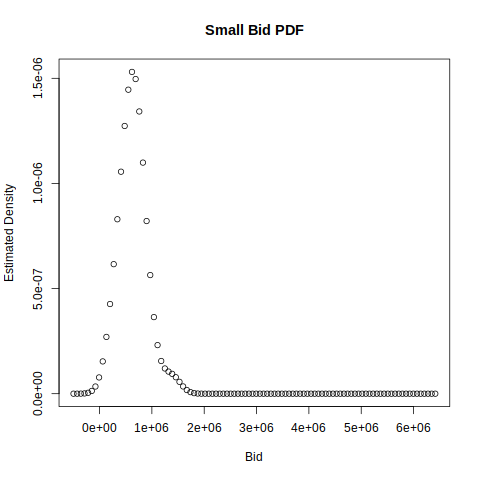
\includegraphics[scale=0.5]{imgs/g_s_median.png}
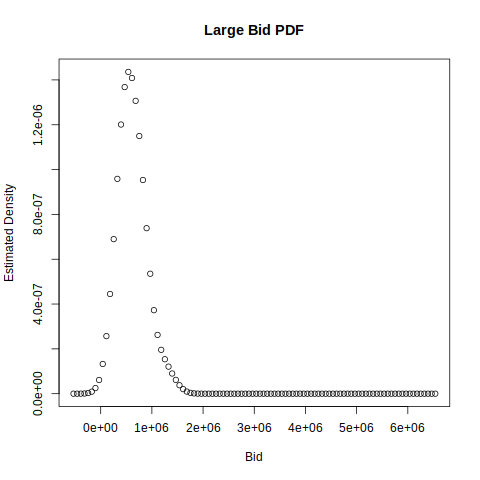
\includegraphics[scale=0.5]{imgs/g_l_median.png}
\end{figure}

While it is counterintuitive that the small businesses actually have a mode
slightly to the right of the large businesses, in our subset of the data the median
small business bid was \$615605 and the median large business bid was \$585513.
The large businesses do have a handful of bids on much larger projects (up to
50 million dollars in the full data set), but they are not present in our
subset of the data.

Even within our subset, the number of large business bids on larger projects
is small enough to not be very visible on the density plots. However,
once we recover the costs, it becomes more noticeable.

\newpage
Similarly, below are the two CDFs of bids (\(G_s\) and \(G_l\) in the above
equation).
\begin{figure}[ht!]
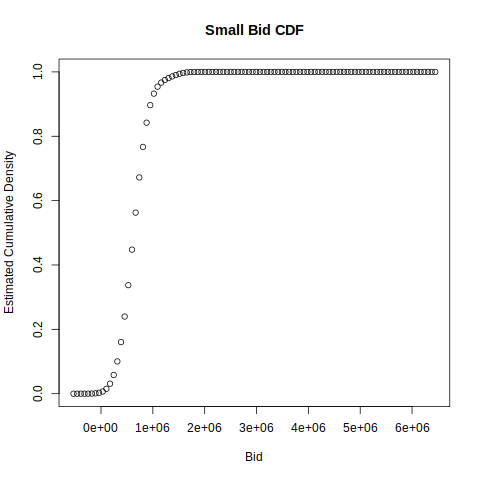
\includegraphics[scale=0.5]{imgs/G_s.png}
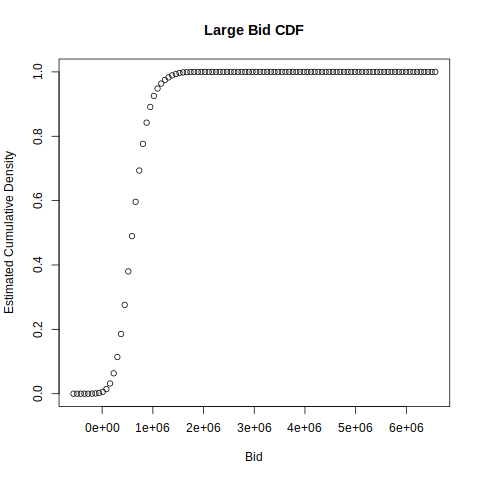
\includegraphics[scale=0.5]{imgs/G_l.png}
\end{figure}

Finally, we calculate the estimated cost distribution by recovering the costs from the bid distribution,
using the equation above (calculated in the Identification section).

%We do not need to condition what we have calculated for the cost distribution on
%the engineers estimate because the bid distribution is already conditioned on it. 

The scale of these plots was set to \$6 million for both small and large
businesses: the reason the small business plots stop much earlier is because
they generally did not participate in auctions for the very large projects,
but rather in auctions where their costs would be smaller (typically under
a million dollars).

\begin{figure}[ht!]
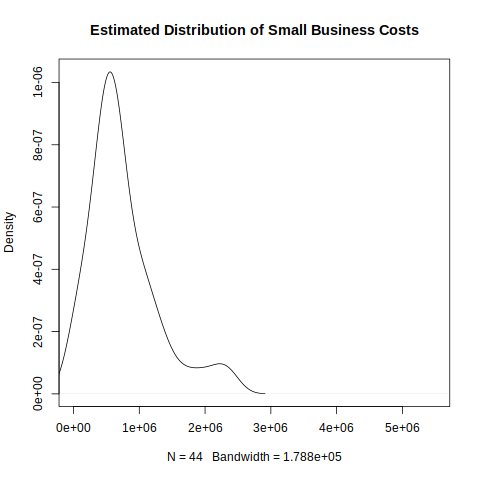
\includegraphics[scale=0.5]{imgs/f_s.png}
%Below is the graph of the PDF for large business on cost. 
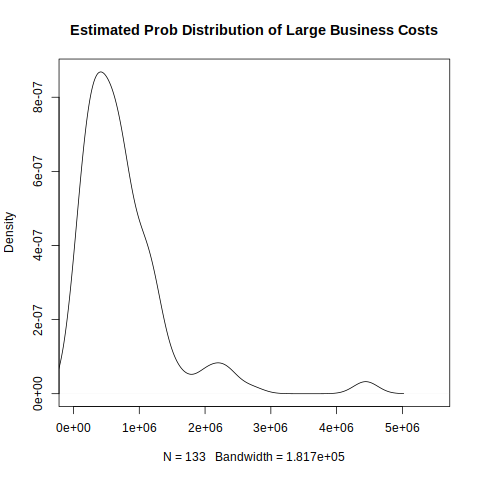
\includegraphics[scale=0.5]{imgs/f_l.png}
\end{figure}

%Below is the graph of the CDF for small business on cost. 
\begin{figure}[ht!]
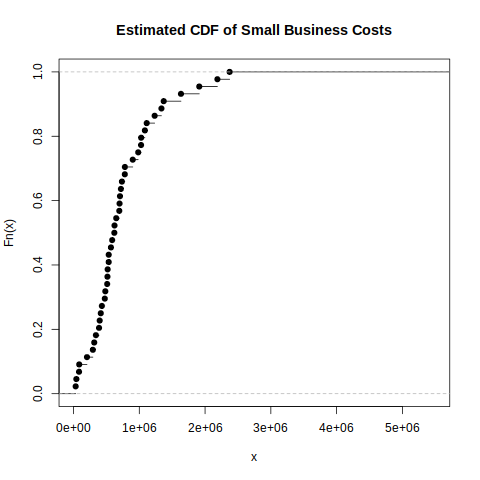
\includegraphics[scale=0.5]{imgs/F_s.png}
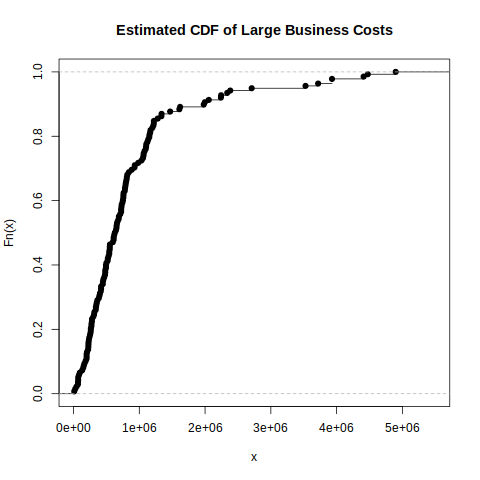
\includegraphics[scale=0.5]{imgs/F_l.png}
\end{figure}
%Below is the graph of the CDF for large business on cost. 

\hspace{10cm}
\newpage
\hspace{5cm}
\newpage
The code used to generate these graphics is below.

\begin{lstlisting}
# n by 2 matrix of n_S and n_L for each i in n
dt_bids <- cbind(calt_full$NumberofSmallBusinessBidders,
                 calt_full$NumberofLargeBusinessBidders)
rows <- c()
for (row_i in seq_len(nrow(dt_bids))) {
  current_row <- dt_bids[row_i, ]
  row_as_char <- paste(current_row, collapse = " ")
  rows <- c(rows, row_as_char)
}
sort(table(rows), decreasing = TRUE)
calt_subset <- calt_full[calt_full$NumberofSmallBusinessBidders == 1 &
                         calt_full$NumberofLargeBusinessBidders == 3, ]

# vectors of large/small bids from our subset
sb_bids_sub <- calt_subset[calt_subset$SmallBusinessPreference == 1, ]$Bid
lb_bids_sub <- calt_subset[calt_subset$SmallBusinessPreference == 0, ]$Bid
# change these further down
ests_subset <- calt_subset$Estimate
# there is just one estimate per auction, so median estimate is same for large/small
median_estimate <- median(ests_subset)
med_est_vec <- rep(median_estimate, length(sb_bids_sub)) # and lb bids too

sb_ests_sub <- calt_subset[calt_subset$SmallBusinessPreference == 1, ]$Estimate
# this is just sb_ests_sub with each entry repeated three times
lb_ests_sub <- calt_subset[calt_subset$SmallBusinessPreference == 0, ]$Estimate

# repeat the median appropriate number of times
sb_med_est_vec <- rep(median_estimate, length(sb_bids_sub))
lb_med_est_vec <- rep(median_estimate, length(lb_bids_sub))

library(hdrcde)
library(devtools)
devtools::install_github("https://github.com/sethmcg/climod")
library(climod)

# cde(x,y) gives p(y|x)
ests_grid <- seq(from = min(sb_ests_sub), to = max(sb_ests_sub), length = 21)
g_l <- cde(lb_ests_sub, lb_bids_sub, deg = 1, link = "log", nxmargin = 21,
           x.name = "Estimates", y.name = "Large Business Bids")
png("./src/imgs/g_l_cond.png")
plot(g_l)
dev.off()

# y is a grid of length 100 plugged in for bids
# z has 100 columns: the third row is those evaluated at the median estimate
png("./src/imgs/g_l_median.png")
plot(g_l$y, g_l$z[3, ]) # at the median estimate
dev.off()
g_s <- cde(sb_ests_sub, sb_bids_sub, deg = 1, link = "log", nxmargin = 21,
           x.name = "Estimates", y.name = "Small Business Bids")
png("./src/imgs/g_s_cond.png")
plot(g_s)
dev.off()
png("./src/imgs/g_s_median.png")
plot(g_s$y, g_s$z[3, ]) # at the median estimate
dev.off()

# we're just taking part of joint PDF, but pdf2cdf can normalize to 1 so it's ok
G_l <- pdf2cdf(g_l$z[3, ], g_l$y)
png("./src/imgs/G_l.png")
plot(G_l)
dev.off()
G_s <- pdf2cdf(g_s$z[3, ], g_s$y)
png("./src/imgs/G_s.png")
plot(G_s)
dev.off()

g_s_spline <- splinefun(g_s$y, g_s$z[3, ])
# integrate(g_s_spline, 100, 6e6) gives 0.996
g_l_spline <- splinefun(g_l$y, g_l$z[3, ])
g_s_s <- g_s_spline(sb_bids_sub)
g_l_l <- g_l_spline(lb_bids_sub)
g_l_s_105 <- g_l_spline(1.05 * sb_bids_sub)
g_s_l_105 <- g_s_spline(lb_bids_sub / 1.05)

G_s_spline <- splinefun(G_s)
G_l_spline <- splinefun(G_l)
G_s_s <- G_s_spline(sb_bids_sub)
G_l_l <- G_l_spline(lb_bids_sub)
G_l_s_105 <- G_l_spline(1.05 * sb_bids_sub)
G_s_l_105 <- G_s_spline(lb_bids_sub / 1.05)

n_S <- 1
n_L <- 3
cost_small <- sb_bids_sub - 1 / (((n_S - 1) * g_s_s) / (1 - G_s_s) + (n_L * g_l_s_105) / (1 - G_l_s_105))
cost_large <- lb_bids_sub - 1 / ((n_S * g_s_l_105) / (1 - G_s_l_105) + ((n_L- 1) * g_l_l) / (1 - G_l_l))

png("./src/imgs/f_s.png")
plot(density(cost_small[cost_small > 0 & is.na(cost_small) == FALSE]),
     main = "Estimated Distribution of Small Business Costs", xlim = c(0, 5.5e6))
dev.off()
png("./src/imgs/f_l.png")
plot(density(cost_large[cost_large > 0 & is.na(cost_large) == FALSE]),
     main = "Estimated Prob Distribution of Large Business Costs", xlim = c(0, 5.5e6))
dev.off()

png("./src/imgs/F_l.png")
plot(ecdf(cost_large[cost_large > 0 & is.na(cost_large) == FALSE]),
     main = "Estimated CDF of Large Business Costs", xlim = c(0, 5.5e6))
dev.off()
png("./src/imgs/F_s.png")
plot(ecdf(cost_small[cost_small > 0 & is.na(cost_small) == FALSE]),
     main = "Estimated CDF of Small Business Costs", xlim = c(0, 5.5e6))
dev.off()
\end{lstlisting}
